\documentclass[11pt]{article}
\usepackage{graphicx}
\usepackage{float}
\usepackage{hyperref}

\begin{document}

\title{An Update on my Machine Translation Work}
\author{Anirudh Srinivasan}
\maketitle
\section{The Encoder-Decoder Model}
\begin{figure}[H]
	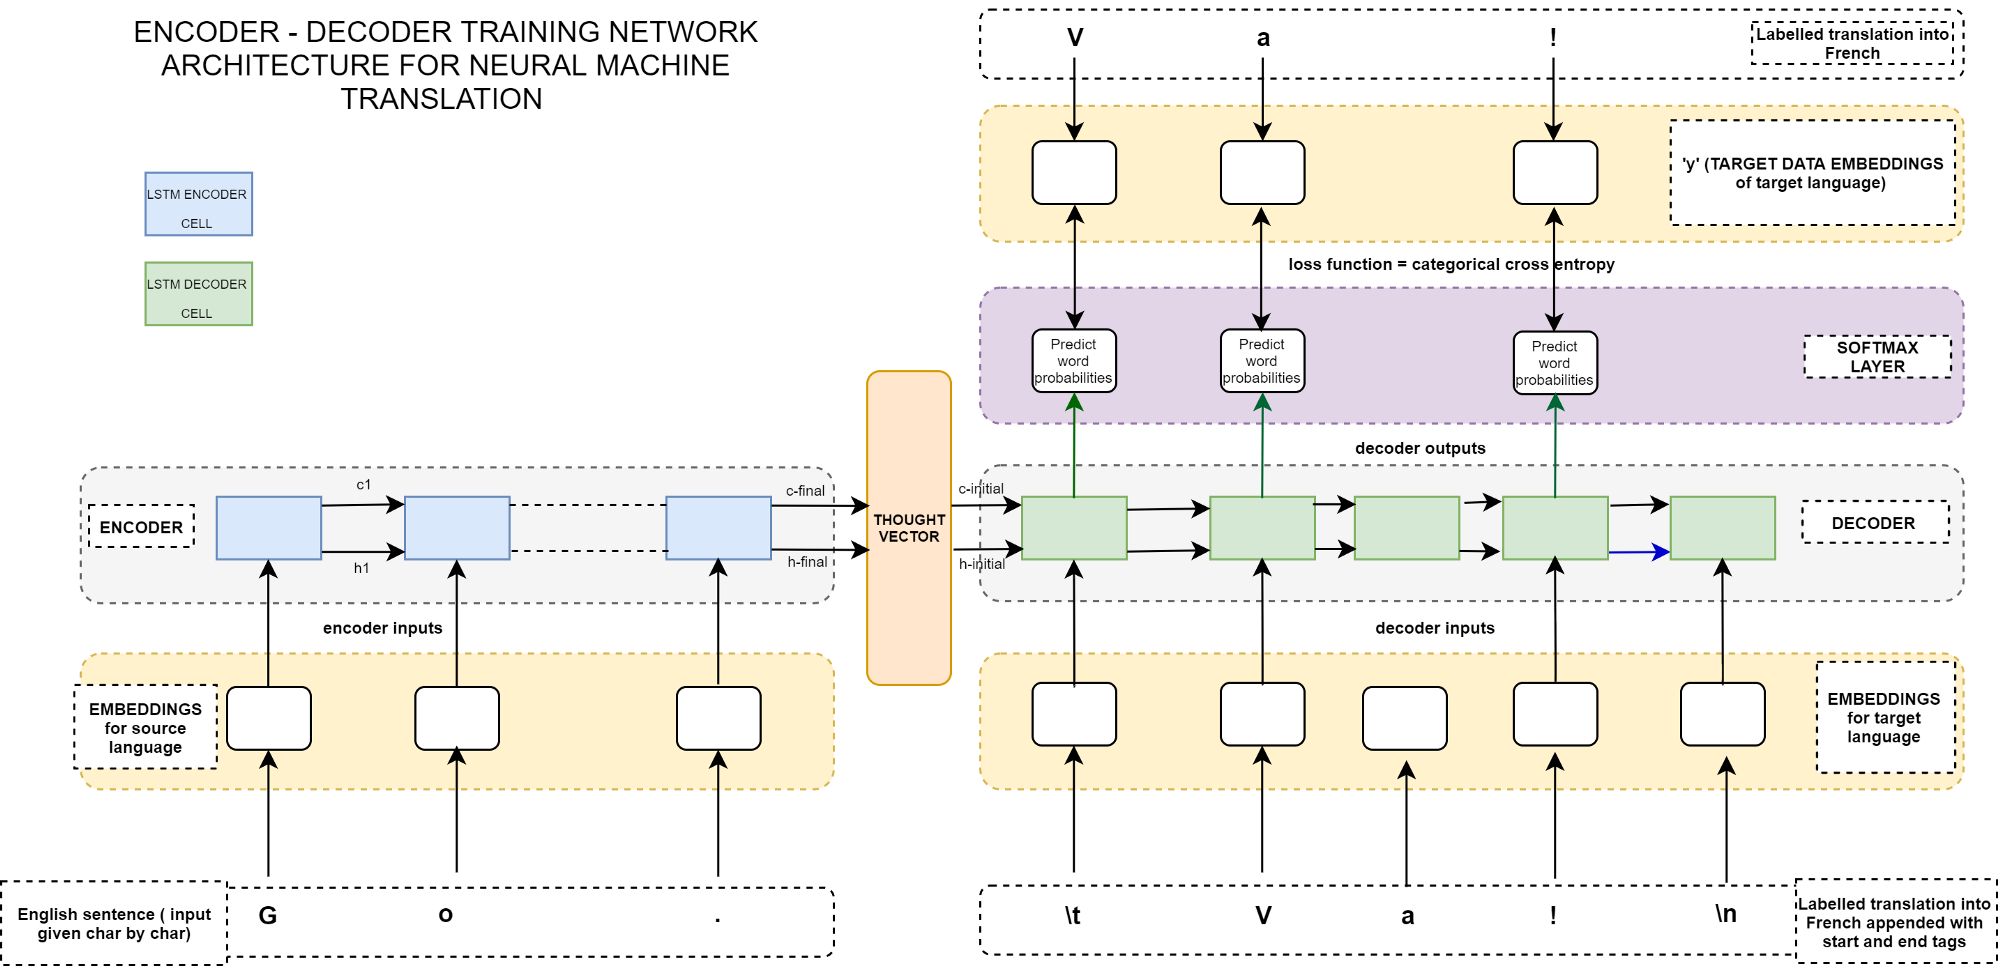
\includegraphics[scale=0.23]{seq2seq.png}
	\caption{Overview of the Model}
\end{figure}

\section{Evaluation Metrics - BLEU}
\begin{itemize}
	\item Cumilative weighted 4 gram overlap
	\item NLTK has an implementation of this ($nltk.translate.bleu\_score$)
	\item Gives score in range [0,1]
	\item Journals report this score multiplied by 100
\end{itemize}

\begin{figure}[H]
	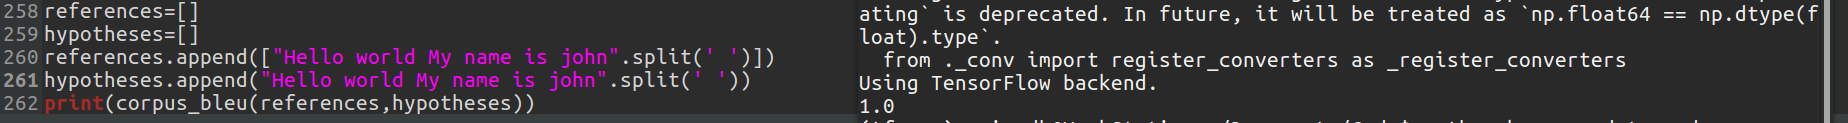
\includegraphics[scale=0.3,trim={0 0 21cm 0},clip]{Screenshot_from_2018-04-02_09-13-25.png}
	\caption{BLEU score of 1}
\end{figure}
\begin{figure}[H]
	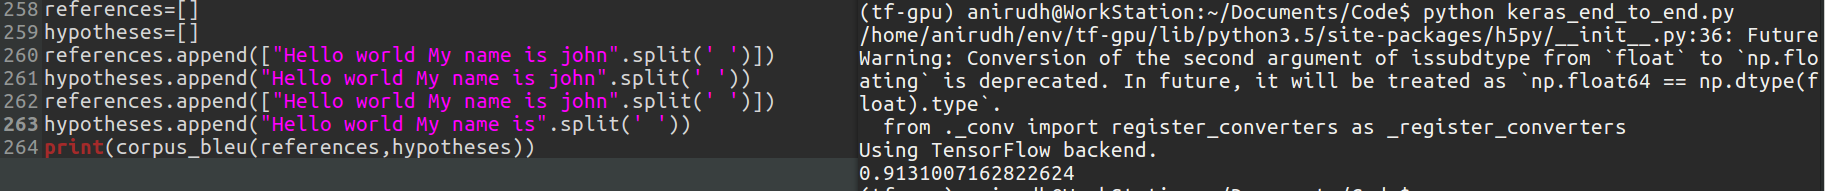
\includegraphics[scale=0.3,trim={0 0 20cm 0},clip]{Screenshot_from_2018-04-02_09-12-17.png}
	\caption{BLEU score smaller than 1}
\end{figure}

\section{Character Level encoding}
\begin{itemize}
	\item Length of LSTM becomes very large
	\item Hidden state of encoder needs to propagate all the way
	\item Not able to capture information for such a long period
	\item Vanishing gradients??
	\item Not feasible to use character level encoding
\end{itemize}

\section{Running Methodology}
\begin{itemize}
					
	\item Create a Model
	\item As of now, using word level encoding
	\item Run it on the fra-eng.txt corpus
	\item Tune the model so that it works well
	\item Run it for the bible sanskrit-english corpus
	      	      	      	      	      
\end{itemize}

\section{Problems discovered}
\begin{figure}[H]
	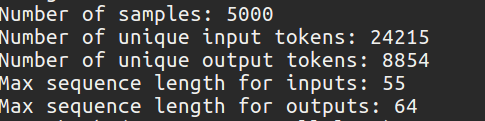
\includegraphics[scale=0.5]{Screenshot_from_2018-04-02_09-31-27.png}
	\caption{Sanskrit}
\end{figure}    
\begin{figure}[H]
	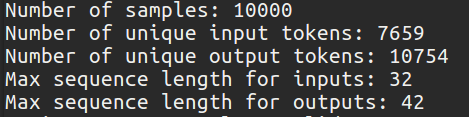
\includegraphics[scale=0.5]{Screenshot_from_2018-04-02_09-32-22.png}
	\caption{French}
\end{figure}

\begin{itemize}
	\item No. of unique tokens in french vs sanskrit
	\item Sentence length in french vs sanskrit
	\item Effective number of samples that one can train on
	\item In sanskrit, there are a large number of words which occur only once. Hence a lot of space get's allocated for them.
	      Some way must be found to handle this
	\item In sanskrit, since sentence length is much more, one pass through the LSTM Takes more time
\end{itemize}


\section{Results so far}
\begin{table}[H]
	\begin{tabular}{|c|c|c|c|}
		\hline
		Corpus         & No. Epochs & BLEU score(test set) & Sample Translation                                                                                          \\ \hline
		fra-eng        & 500        & 0.0219               & \href{run:/run/user/1000/gvfs/sftp:host=172.16.5.90/home/anirudh/Documents/Code/1522663802.txt}{Click Here} \\ \hline
		Sanskrit Bible & 100        & 0.0115               & \href{run:/run/user/1000/gvfs/sftp:host=172.16.5.90/home/anirudh/Documents/Code/1522733179.txt}{Click Here} \\ \hline
		Sanskrit Bible & 500        & 0.0026               & \href{run:/run/user/1000/gvfs/sftp:host=172.16.5.90/home/anirudh/Documents/Code/1522687677.txt}{Click Here} \\ \hline
	\end{tabular}
	\caption{BLEU scores for fra-eng and Sanskrit Bible Corpus}
\end{table}

The above scores suggest that the model may be overfitting

\begin{table}[H]
	\begin{tabular}{|c|c|c|}
		\hline
		No. Epochs & BLEU score on train set & BLEU score on test set \\ \hline
		10         & 0.1286                  & 0.1243                 \\ \hline
		20         & 0.0143                  & 0.0058                 \\ \hline
		50         & 0.0513                  & 0.0290                 \\ \hline
	\end{tabular}
	\caption{BLEU scores for test and train set on Sanskrit Bible Corpus}
\end{table}


\begin{itemize}
					
	\item BLEU scores, even for fra-eng were very low. Common papers report BLEU scores of around 30(multiplied by 100)
	\item As the number of epochs were increased, the output sentences made more sense w.r.t the expected output
	\item In current implementation, there are few constraints w.r.t the length of the input and output sentence
	\item This model was designed in such a way that the length of the sentence shouldn't be a Problems
	\item Will modify the code and try that
\end{itemize}

\section{Future Prospects}
\begin{itemize}
	\item Vectors used for input and output are very sparse, because there are a large number of words
	\item Propose a new vector scheme
	\item Use a POS tagger$(INRIA, France)$ to extract the root word and POS
	\item Let the vocabulary contain the root words alone. To the one-hot-vectors, add the POS information as features
\end{itemize}
\subsection{word2vec/GloVe}
\begin{itemize}
	\item word2vec was attempted using the original implementation from Google
	\item It did not parse the input correctly. The input had words separated by spaces
	\item It should have taken each word as a unit and split
	      based on spaces. Instead, it took each character as a unit and ran the algorithm for it
	\item The implementation was done in C and probably doesn't take into account characters that are non ASCII. Will look into it later
\end{itemize}
\end{document}